\section{Experimental results}
\label{exp}


\textcolor{red}{SECTION REECRITE POUR ICRA}


The proposed method has been validated on HRP-2 using the following
scenarii: the robot executes a long trajectory in an environment
cluttered by obstacles located along the robot path. The followed path
is a $6\text{x}4 \mathrm{m}$ square such as the position ends at its
starting point.

This setup demonstrates that the execution using this control scheme
is precise and reliable. The robot reaches its goal position with an
error of a few centimeters whereas open loop control schemes is off by
more than a meter. Moreover, the control scheme is reliable: it takes
more than a minute for the robot to reach its goal point. During that
time, the localization precision can change, the robot position can be
lost, \ldots The control scheme is designed to be robust toward these
situations as illustrated by the video.


This experiment uses the pattern generator described by
\cite{10icra.perrin} and the stack of tasks formalism
\cite{09icar.mansard} to implement the control scheme. The pattern
generator provides reference trajectories for the center of mass and
the feet. Trajectory following tasks for these particular bodies are
then inserted into the control framework. The solver will then realize
implicitly the inverse geometry computations required to recompute the
whole-body trajectory and simplifies the actual control scheme.


\begin{figure}[ht!]
  \begin{center}
    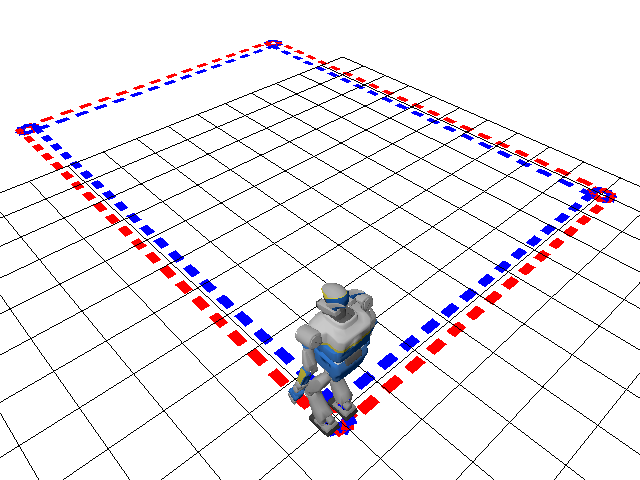
\includegraphics[width=0.45\textwidth]{fig/demo.png}
  \end{center}
  \caption{HRP-2 experiment scenario. The robot position is both
    its starting and final position. \label{fig:scenario}}
\end{figure}


Fig.~\ref{fig:following} illustrates the experiment on the real
robot. This experiment video is available on the
web\footnote{\mbox{\url{http://homepages.laas.fr/tmoulard/video/11icra-tmoulard.mp4}}}. Fig.~\ref{fig:scenario}
provides an overview of the scenario: the rectangle on the left
symbolizes the initial position and the rectangle on the right the
final position.


\begin{figure}[ht!]
  \begin{center}
    \begin{tabular}{|c|c|c|}
      \hline
      \bf{Strategy} & Replanning & Correction\\
      \hline
      \bf{CPU usage}          & High     & Low (real-time)\\
      \bf{Reactivity}         & Low      & High\\
      \bf{Position filtering} & Explicit & Implicit\\
      \hline
    \end{tabular}
  \end{center}
  \caption{Comparison of replanning and online correction when
    compensating for execution errors. \label{fig:comparison}}
\end{figure}


This work has been motivated by the previous experimental setup
described in \cite{11humanoids.baudouin}. In this paper, fast online
replanning is used to handle changes in the environment. Using
replanning to absorb the drift has been considered at first but
suffers from several drawbacks. The initial idea by using replanning
is stating that if the planning can be accelerated enough, there is no
need to take into account the execution errors as it can be handled by
changing the robot starting position to its real one instead of the
planned one and regenerating the trajectory which is yet to be
executed. This is difficult in practice for several reasons. First
using the localization system as an input of the planning component is
dangerous. If the localization is bad, so will be the plan. Therefore,
it is required to filter the robot position explicitly to ensure a
high quality localization at every point of time. On the opposite, as
our control scheme only modifies the next step and is bounded by a
correction limit, a low-pass filter is implicitly applied and
protects the control scheme from temporary erroneous
localization. Second, if the localization is imprecise and is near an
obstacle, the estimated position may be in collision with the
obstacle. Even if this is possible to project the position outside of
the obstacle, this additional step renders the replanning harder to
implement and understand. To finish, even if fast replanning is
possible, random planning such as RRT-based methods cannot be used
efficiently in a real-time context. An heuristic has been defined in
\cite{11humanoids.baudouin} indicating that when a replanning starts,
it starts three steps after the current position so that there is a
high probability that the planning ends before the robot executes
this step. It means that the correction will not be reactive and that
it may be too late when the correction is taken into account.  On the
opposite, this control scheme could provide correction at each
iteration of the control loop and could even modify the trajectory of
the swinging foot during a step. This has not been implemented as the
current strategy already provides satisfying results but it would
definitely be an interesting enhancement for a future work.


\FloatBarrier

%%% Local Variables:
%%% ispell-local-dictionary: "american"
%%% LocalWords:
%%% End:
